\documentclass[a4paper]{article}

    % Caracteres
    \usepackage[francais]{babel} % Typographie française
    \usepackage[utf8]{inputenc} % Caractères en UTF-8
    \usepackage[T1]{fontenc} % Fontes Extended Computer modern (EC)
    
    % Images
    \usepackage{graphicx} % Inclure des images
    \usepackage{float} % Placer les figures dans une page
    %\usepackage{wrapfig} % Placer les figures dans un texte
    % \usepackage{caption}
    
    % En-tete et pieds de page
    \usepackage{fancyhdr} % Inclure en-tetes et pieds de pages
    \usepackage{lastpage} % Indiquer le nombre de pages totals
    
    % Liens
    \usepackage[unicode]{hyperref} % Inclure des liens externes
    %\hypersetup{colorlinks, linkcolor=black, urlcolor=blue} % Change la couleur des liens

    % Code
    \usepackage{listings} % Inclure du code
    % \usepackage{comment} % Commentaires sur plusieurs lignes
    
    \title{Manuel d'utilisateur d'ACCECS}
    \author{Alexis Giraudet \and Asma Khelifi \and Jean-Christophe Guérin \and Geoffrey Desbrosses \and Léo Cassiau \and Tantely Randriamaharavomanana \and Ugo Mahey}
    \date\today

\begin{document}

\maketitle

\tableofcontents
\newpage

\section{Préface}
\subsection{Public visé}
    Ce document est destiné aux utilisateurs du logiciel Assistance for the Construction of Critical
Embedded Control Systems (ACCECS). ACCECS fonctionne sur la plupart des systèmes de type Unix et Windows ayant java d'installé. 
    
    Ce document regroupant un tutoriel d'utilisation d'ACCECS et son manuel utilisateur, est destiné à plusieurs types d'utilisateurs :
    \begin{description}
        \item[Novice] Notre logiciel vous intéresse mais vous ne savez pas de quoi il en retourne ? Commencez par la section \nameref{sec:presentation}.
        \item[Utilisateur averti] Vous souhaitez installer notre logiciel et l'essayer ? Il faut alors vous référer à la section \nameref{sec:utilisation}.
        \item[Développeur] Ce projet vous intéresse et vous souhaitez modifier son fonctionnement ? Reportez-vous à la section \nameref{sec:avance}.
    \end{description}

    Enfin, ce document étant réalisé dans le cadre d'un projet universitaire, il est libre de droits.
    
\subsection{Présentation du projet ACCECS}\label{sec:presentation}

    Le logiciel ACCECS est issu d'un projet réalisé dans un cadre universitaire, par des élèves de deuxième année du master ALMA, à la \footnote{\url{http://www.univ-nantes.fr/}}{faculté des sciences et techniques de Nantes}. L'objectif de ce projet est de mettre en \oe uvre les différentes connaissances acquises durant nos différents cours afin d'atteindre un but définit en équipe. Ce projet est encadré par M. \footnote{http://pagesperso.lina.univ-nantes.fr/~attiogbe-c/}{Attiogbe} et M. \footnote{http://pagesperso.lina.univ-nantes.fr/~andre-p/fr/index.html}{André}, tous les deux enseignant-chercheur travaillant au \footnote{https://www.lina.univ-nantes.fr/}{Laboratoire Informatique de Nantes Atlantique (LINA)}.

\subsection{Qu'est ce qu'ACCECS ?}

    L'objectif du projet est de réaliser, en équipe, un outil facilitant la rédaction des programmes utilisant la méthode B. La méthode B est une méthode formelle permettant d'assurer le bon fonctionnement des programmes, et notamment dans le cas qui nous intéresse ici, les programmes présents sur les systèmes embarqués. Ces systèmes possèdent des actuateurs et des senseurs, qui permettent de prendre connaissance et d'agir sur l'environnement du système. Ceci nous permet de commencer à décrire le comportement du système, appelé le contrôleur. C'est donc à partir la spécification du système embarqué que l'on commence à rédiger le programme du contrôleur. Notre outil a pour but de faciliter le passage entre la spécification du système et la spécification du contrôleur.

\section{Utilisation de base}\label{sec:utilisation}
\subsection{Installation}
Ce projet est avant tout un projet expérimental, de ce fait l'utilisation de l'outil ACCECS n'est pas standardisée.

\subsubsection{Lien du dépôt des sources}
    Le lien suivant contient le code source en libre accès :
    \url{https://github.com/Giraudux/ACCECS}

\subsubsection{Lancer le serveur}
    Pour lancer le serveur qui accueille les requêtes de l'interface web, tapez la commande suivante dans le répertoire racine :
    \begin{lstlisting}
        mvn jetty:run
    \end{lstlisting}
    
    Une fois le serveur lancé, vous pouvez accéder à l'interface à l'adresse suivante :
    \url{localhost:8080}

\subsection{Génération d'un squelette de machine B}
    Cette section montre comment utiliser simplement notre outil.
    
\subsubsection{Énumération des différents types}
    
    \begin{figure}[ht]
        \centering
        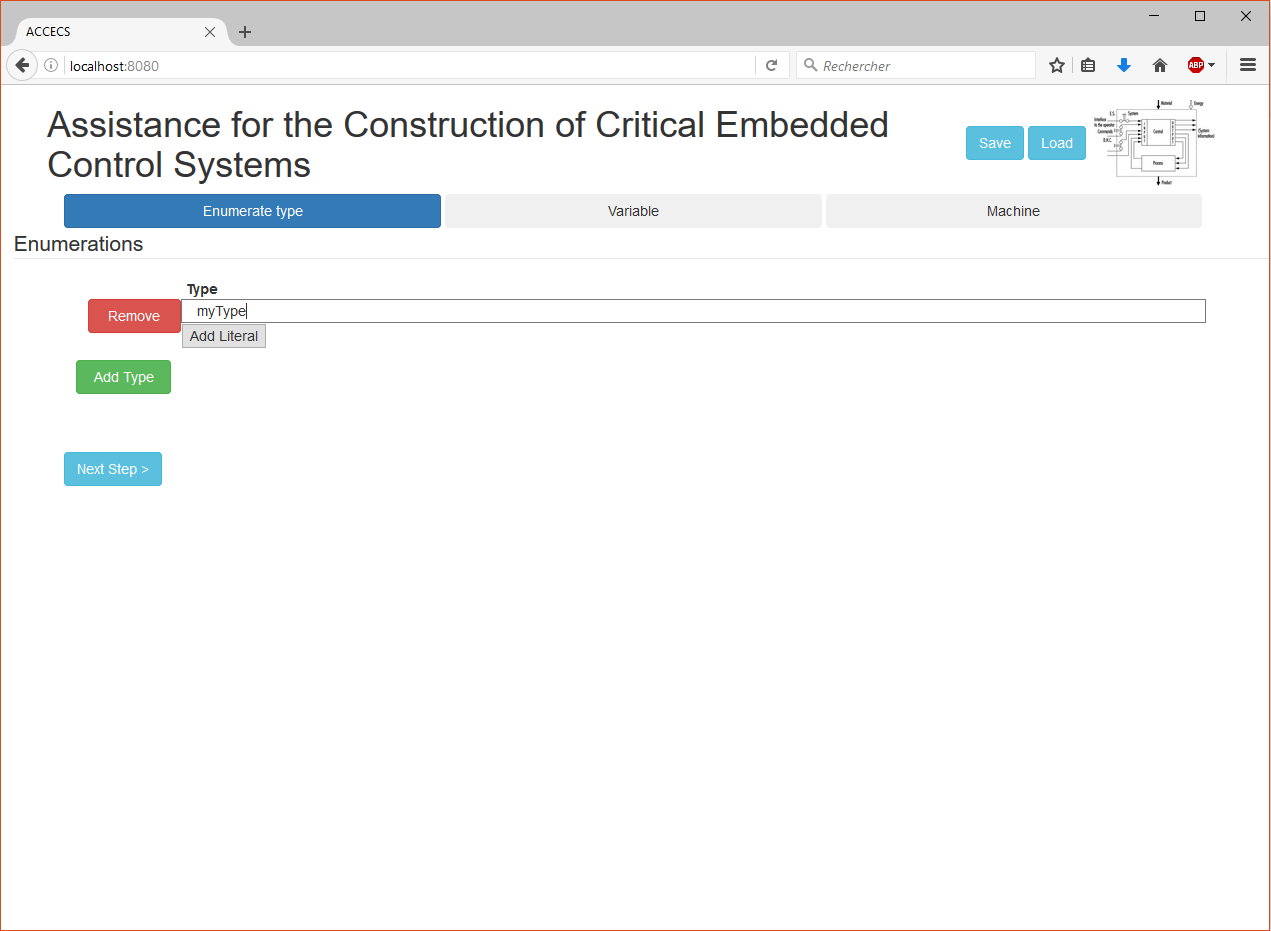
\includegraphics[width=\textwidth]{screen1.png}
        \caption{Capture d'écran de la page 1}
        \label{fig:screen1}
    \end{figure}
    
    La première page d'ACCECS permet de spécifier des nouveaux types. Ici, un seul nouveau type est déclaré. Une fois la liste des nouveaux types déclarés, on passe à l'étape suivante.
    
\subsubsection{Déclarations des variables et des propriétés du système}
    Cette page permet de déclarer la liste des variables de notre système, ainsi que les propriétés du système, que l'on a appelé ici invariant's property pour lever toutes ambiguïtés. Une variable a un nom, un type, une catégorie, un intervalle de valeurs possibles et une valeur par défaut. La valeur par défaut est par défaut mis à 0 pour un entier. L'image en haut à droite est là pour aider à comprendre la correspondance des variables avec ce que l'utilisateur doit rentrer comme données.
    
    \begin{figure}[ht]
        \centering
        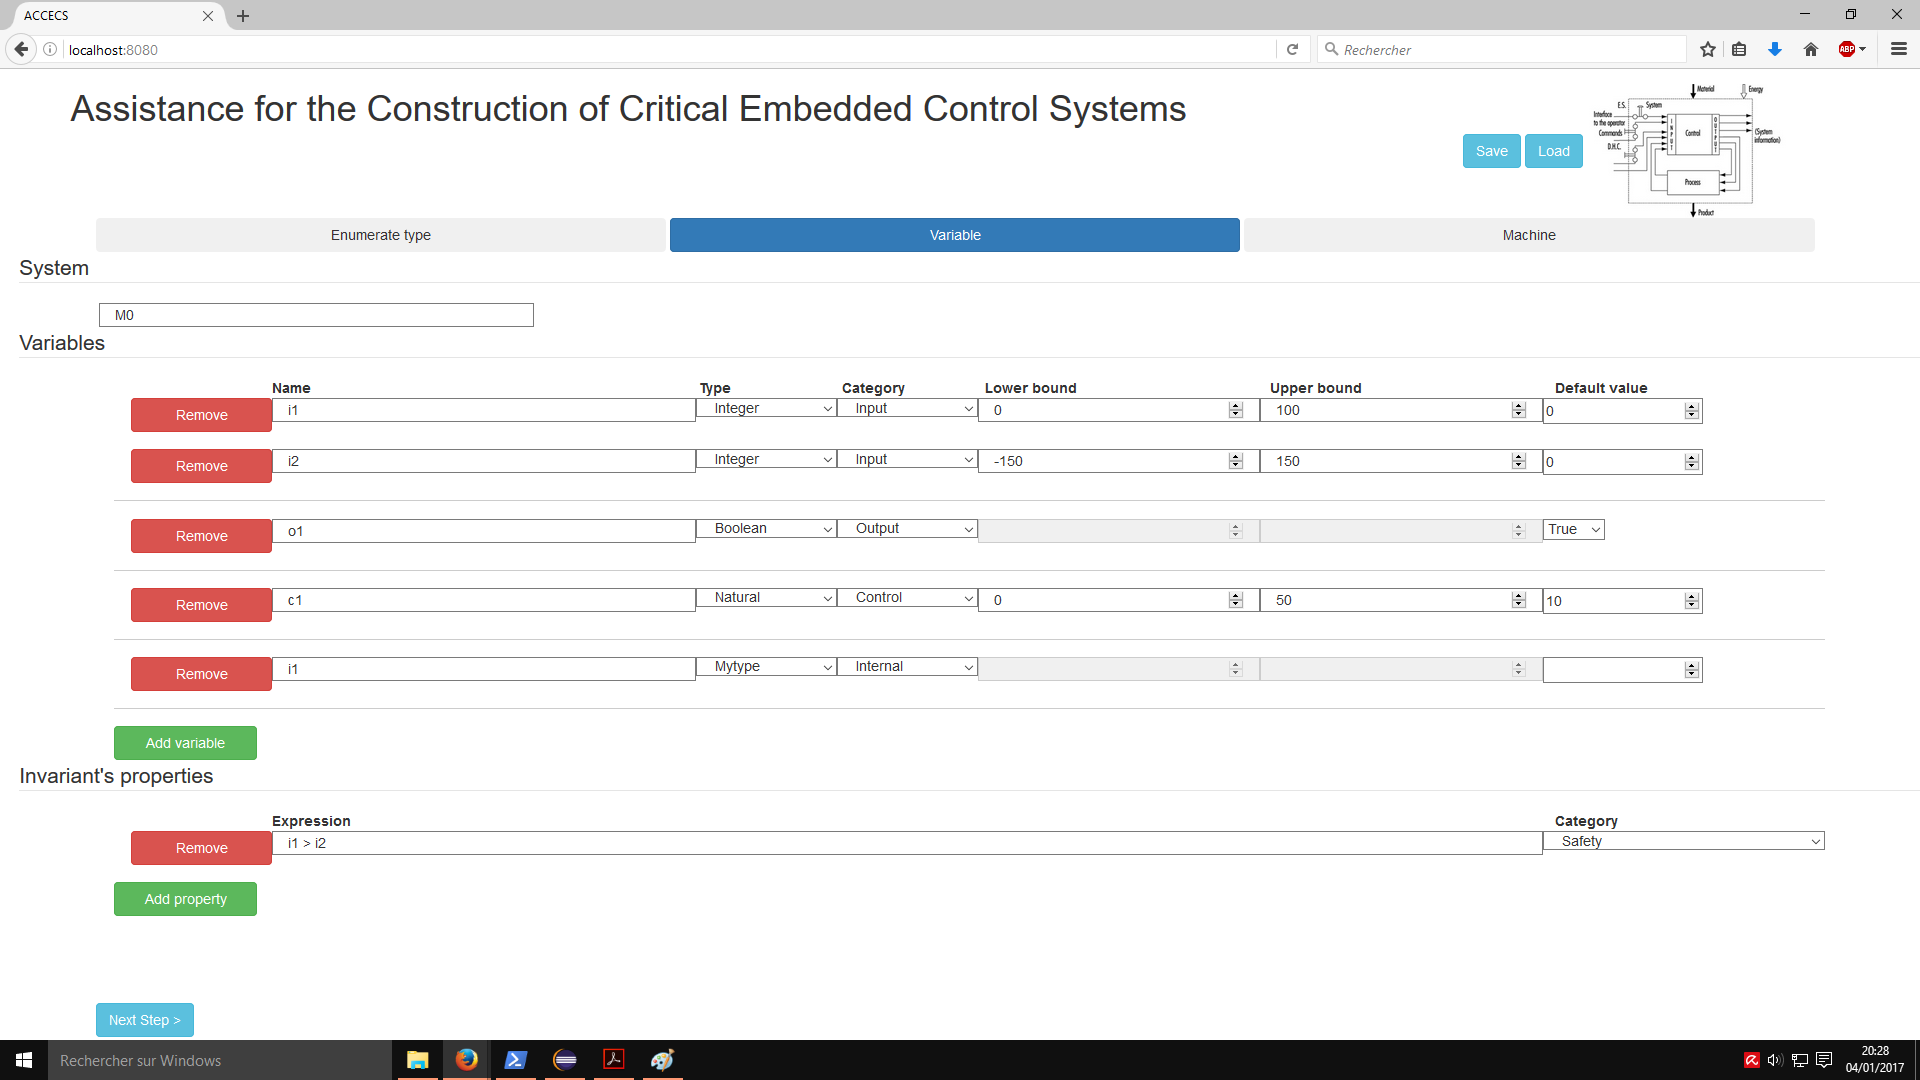
\includegraphics[width=\textwidth]{screen2.png}
        \caption{Capture d'écran de la page 2}
        \label{fig:screen2}
    \end{figure}
    
    Il est possible à tout moment d'enregistrer les données présentes sur cette page avec les boutons save et load en haut à droite.
    
\subsubsection{Squelette généré}
    Enfin, sur la dernière figure \ref{fig:screen3} on peut voir le squelette B généré, avec les variables, les invariants, etc\dots Au besoin, on peut régénérer le squelette ou appuyer sur des boutons pour copier/coller plus simplement le code généré.
    
    \begin{figure}[ht]
        \centering
        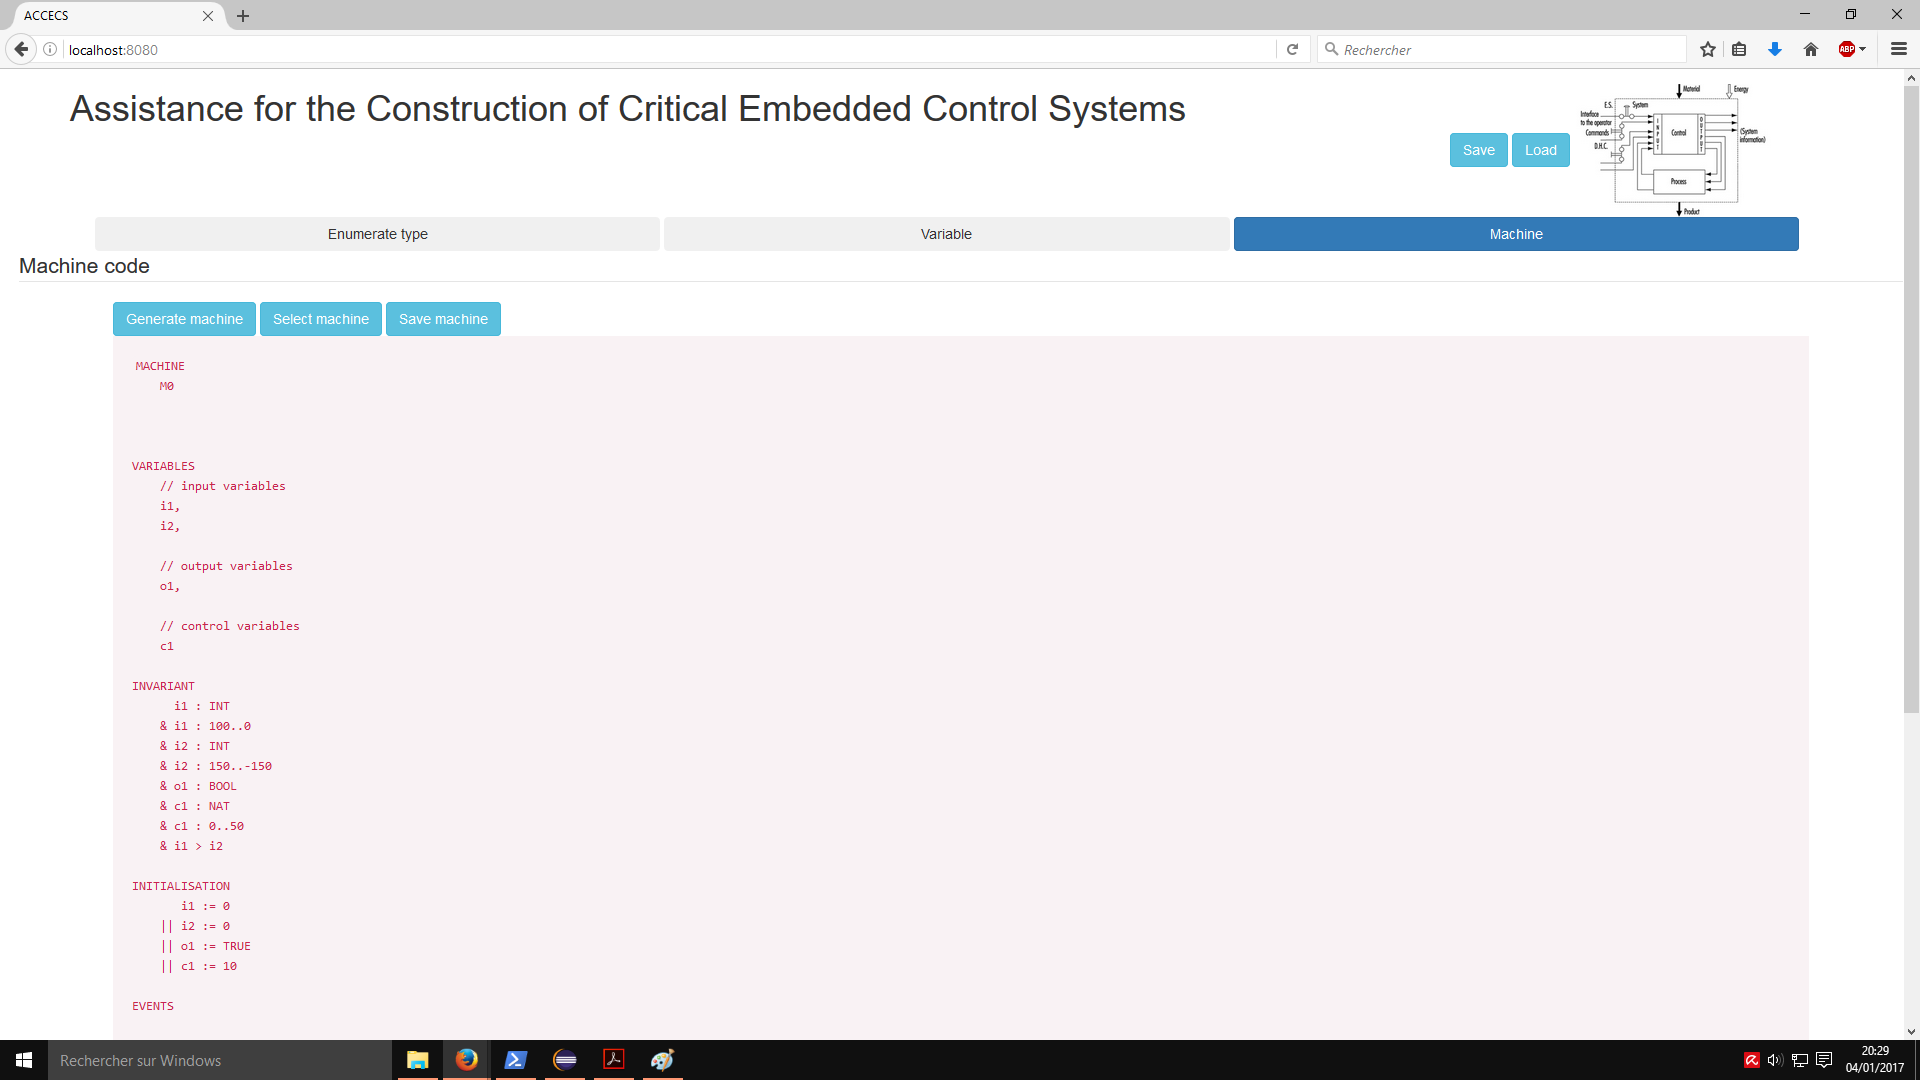
\includegraphics[width=\textwidth]{screen3.png}
        \caption{Capture d'écran de la page 3}
        \label{fig:screen3}
    \end{figure}
    

\newpage{}

\section{Sujets avancés}\label{sec:avance}
    Cette partie s'attarde sur les questions soulevées durant la conception de l'outil ACCECS. Cette section abordera de nombreuses notions relatives à la méthode B, il est donc préférable d'être à l'aise avec les notions des méthodes formelles avant de lire la suite.
    
\subsection{Les outils développement}
	Le sujet du projet nous laissait choisir les différentes technologies à manipuler pour réaliser l'outil ACCECS. Cette partie s'attarde sur ces choix et les explique.
    
\subsubsection{Une interface web}
	Après plusieurs discussions avec le corps enseignant, une des premières nécessités était de de rendre l'outil accessible facilement, si possible depuis internet et utilisable par plusieurs usagers en même temps. En effet, l'outil serait amené à être utilisé par des équipes, et les résultats de l'outil doivent être accessibles facilement aux différent membres de l'équipe. Nous avons donc choisi d'utiliser une interface web.
	
	\bigskip
	
	Nous avons choisi d'utiliser bootstrap pour un meilleur rendu en CSS, et car c'est une bibliothèque populaire. Les scripts sont rédigés en simple javascript car c'est une partie assez minime du projet, la plupart des calculs étant fait à l'aide de Java. Enfin, nous avons utilisé Jetty comme serveur par défaut, car il est facile d'utilisation (sous forme de plugin maven).
	
\subsubsection{Le langage utilisée : Java}
    L'essentiel du code est écrit en Java, car c'est le langage sur lequel les membres de l'équipe étaient le plus à l'aise. De plus, grâce aux servlets, il est facile de lier l'interface web et notre code source. Enfin, les de classe de Java permettent de regrouper certaines notions du B. Maven est également utilisé pour gérer facilement les dépendances et faciliter la reprise du projet.

\subsubsection{Le format des données : JSON}
    Nous avons choisi de représenter les données échangées entre l'interface et le code source sous le format JSON, car c'est un format facile à lire et à manipuler, avec des analyseurs syntaxiques disponibles facilement, notamment sur le web. C'est sous ce format que sont enregistrées les données rentrées par l'utilisateur. On peut ainsi enregistrer ces données, créer des jeux de données, les échanger, et les rouvrir sous une autre machine. 

\subsubsection{Le moteur de template Jtwig}
    Les résultats fournis par notre outil se doivent de respecter un squelette correspondant à une machine B. Pour modifier facilement le squelette selon nos besoins, nous avons choisi d'utiliser un moteur de template. Jtwig est l'un d'eux, qui s'avère simple d'utilisation, très complet, compatible avec Java et assez populaire pour espéré qu'il soit maintenu dans les années à venir. 

\subsection{La limite entre notre outil et la méthode B}
    Notre outil a pour but d'aider à démarrer la conception d'une machine B. L'une des principales difficultés du projet a été de déterminer la fin.
    
\subsubsection{Différencier un contrôleur et la future machine B}
    L'un des premiers besoins exprimé par le corps enseignant était que notre outil ne soit pas automatiquement associé à la méthode B. Il doit avant tout servir à spécifier un contrôleur qui va agir sur son environnement. Ce contrôleur possède des actuateurs, des senseurs, etc\dots qui vont servir à définir les premières variables de base. Notre interface doit donc permettre de rentrer ces premières variables ainsi que les premières propriétés déduites uniquement des propriétés du contrôleur, le tout de la manière la plus intuitive celui qui manipule le contrôleur, et non pour celui qui sera amené à rédiger le code en B.
    
\subsubsection{Les évènements}
    Les évènements sont des opérations qui se déclenchent lorsqu'un senseur détecte une valeur critique. On peut déduire des évènements des variables de base indiqués par l'utilisateur, afin de les générer leurs squelettes dans la future machine B. Les variables d'entrées (input) génère ainsi des événements sensoriels (sense) et les variables de sortie (output) génèrent des événements de réactions (reaction). Il existe deux dernières catégories d'événements, ceux de surveillance (monitor) et ceux de contrôles (control). Les événements de contrôles lisent en entrée les variables de contrôles et agissent sur les variables de sortie, tandis que les événements de surveillance lisent les variables d'entrées et agissent sur les variables de contrôles. Il n'est pas possible de générer un squelette pour ces deux types d'événements car les variables de sorties et d'entrées sont impossibles à prévoir.
    
\subsubsection{Les limites liées à la complexité du B}
    La méthode B elle-même s'est avéré être un frein, le but d'ACCECS étant de faciliter le début de la spécification d'une machine B, mais pas d'essayer de remplacer la méthode elle-même. Nous avons donc choisi de ne pas rendre lisible par notre outil du code en B. Cela demanderait de recoder toutes les notions de B en java pour un résultat sûrement de qualité moindre, et un suivi serait nécessaire en fonction des mises à jour du B. Cela représente un travail imposant pour un résultat moindre, car il est vrai que notre outil facilite la maintenance du code B, mais il se veut rester basique.
    
\end{document}
